% Options for packages loaded elsewhere
\PassOptionsToPackage{unicode}{hyperref}
\PassOptionsToPackage{hyphens}{url}
\PassOptionsToPackage{dvipsnames,svgnames,x11names}{xcolor}
%
\documentclass[
  letterpaper,
  DIV=11,
  numbers=noendperiod]{scrartcl}

\usepackage{amsmath,amssymb}
\usepackage{iftex}
\ifPDFTeX
  \usepackage[T1]{fontenc}
  \usepackage[utf8]{inputenc}
  \usepackage{textcomp} % provide euro and other symbols
\else % if luatex or xetex
  \usepackage{unicode-math}
  \defaultfontfeatures{Scale=MatchLowercase}
  \defaultfontfeatures[\rmfamily]{Ligatures=TeX,Scale=1}
\fi
\usepackage{lmodern}
\ifPDFTeX\else  
    % xetex/luatex font selection
\fi
% Use upquote if available, for straight quotes in verbatim environments
\IfFileExists{upquote.sty}{\usepackage{upquote}}{}
\IfFileExists{microtype.sty}{% use microtype if available
  \usepackage[]{microtype}
  \UseMicrotypeSet[protrusion]{basicmath} % disable protrusion for tt fonts
}{}
\makeatletter
\@ifundefined{KOMAClassName}{% if non-KOMA class
  \IfFileExists{parskip.sty}{%
    \usepackage{parskip}
  }{% else
    \setlength{\parindent}{0pt}
    \setlength{\parskip}{6pt plus 2pt minus 1pt}}
}{% if KOMA class
  \KOMAoptions{parskip=half}}
\makeatother
\usepackage{xcolor}
\setlength{\emergencystretch}{3em} % prevent overfull lines
\setcounter{secnumdepth}{-\maxdimen} % remove section numbering
% Make \paragraph and \subparagraph free-standing
\ifx\paragraph\undefined\else
  \let\oldparagraph\paragraph
  \renewcommand{\paragraph}[1]{\oldparagraph{#1}\mbox{}}
\fi
\ifx\subparagraph\undefined\else
  \let\oldsubparagraph\subparagraph
  \renewcommand{\subparagraph}[1]{\oldsubparagraph{#1}\mbox{}}
\fi

\usepackage{color}
\usepackage{fancyvrb}
\newcommand{\VerbBar}{|}
\newcommand{\VERB}{\Verb[commandchars=\\\{\}]}
\DefineVerbatimEnvironment{Highlighting}{Verbatim}{commandchars=\\\{\}}
% Add ',fontsize=\small' for more characters per line
\usepackage{framed}
\definecolor{shadecolor}{RGB}{241,243,245}
\newenvironment{Shaded}{\begin{snugshade}}{\end{snugshade}}
\newcommand{\AlertTok}[1]{\textcolor[rgb]{0.68,0.00,0.00}{#1}}
\newcommand{\AnnotationTok}[1]{\textcolor[rgb]{0.37,0.37,0.37}{#1}}
\newcommand{\AttributeTok}[1]{\textcolor[rgb]{0.40,0.45,0.13}{#1}}
\newcommand{\BaseNTok}[1]{\textcolor[rgb]{0.68,0.00,0.00}{#1}}
\newcommand{\BuiltInTok}[1]{\textcolor[rgb]{0.00,0.23,0.31}{#1}}
\newcommand{\CharTok}[1]{\textcolor[rgb]{0.13,0.47,0.30}{#1}}
\newcommand{\CommentTok}[1]{\textcolor[rgb]{0.37,0.37,0.37}{#1}}
\newcommand{\CommentVarTok}[1]{\textcolor[rgb]{0.37,0.37,0.37}{\textit{#1}}}
\newcommand{\ConstantTok}[1]{\textcolor[rgb]{0.56,0.35,0.01}{#1}}
\newcommand{\ControlFlowTok}[1]{\textcolor[rgb]{0.00,0.23,0.31}{#1}}
\newcommand{\DataTypeTok}[1]{\textcolor[rgb]{0.68,0.00,0.00}{#1}}
\newcommand{\DecValTok}[1]{\textcolor[rgb]{0.68,0.00,0.00}{#1}}
\newcommand{\DocumentationTok}[1]{\textcolor[rgb]{0.37,0.37,0.37}{\textit{#1}}}
\newcommand{\ErrorTok}[1]{\textcolor[rgb]{0.68,0.00,0.00}{#1}}
\newcommand{\ExtensionTok}[1]{\textcolor[rgb]{0.00,0.23,0.31}{#1}}
\newcommand{\FloatTok}[1]{\textcolor[rgb]{0.68,0.00,0.00}{#1}}
\newcommand{\FunctionTok}[1]{\textcolor[rgb]{0.28,0.35,0.67}{#1}}
\newcommand{\ImportTok}[1]{\textcolor[rgb]{0.00,0.46,0.62}{#1}}
\newcommand{\InformationTok}[1]{\textcolor[rgb]{0.37,0.37,0.37}{#1}}
\newcommand{\KeywordTok}[1]{\textcolor[rgb]{0.00,0.23,0.31}{#1}}
\newcommand{\NormalTok}[1]{\textcolor[rgb]{0.00,0.23,0.31}{#1}}
\newcommand{\OperatorTok}[1]{\textcolor[rgb]{0.37,0.37,0.37}{#1}}
\newcommand{\OtherTok}[1]{\textcolor[rgb]{0.00,0.23,0.31}{#1}}
\newcommand{\PreprocessorTok}[1]{\textcolor[rgb]{0.68,0.00,0.00}{#1}}
\newcommand{\RegionMarkerTok}[1]{\textcolor[rgb]{0.00,0.23,0.31}{#1}}
\newcommand{\SpecialCharTok}[1]{\textcolor[rgb]{0.37,0.37,0.37}{#1}}
\newcommand{\SpecialStringTok}[1]{\textcolor[rgb]{0.13,0.47,0.30}{#1}}
\newcommand{\StringTok}[1]{\textcolor[rgb]{0.13,0.47,0.30}{#1}}
\newcommand{\VariableTok}[1]{\textcolor[rgb]{0.07,0.07,0.07}{#1}}
\newcommand{\VerbatimStringTok}[1]{\textcolor[rgb]{0.13,0.47,0.30}{#1}}
\newcommand{\WarningTok}[1]{\textcolor[rgb]{0.37,0.37,0.37}{\textit{#1}}}

\providecommand{\tightlist}{%
  \setlength{\itemsep}{0pt}\setlength{\parskip}{0pt}}\usepackage{longtable,booktabs,array}
\usepackage{calc} % for calculating minipage widths
% Correct order of tables after \paragraph or \subparagraph
\usepackage{etoolbox}
\makeatletter
\patchcmd\longtable{\par}{\if@noskipsec\mbox{}\fi\par}{}{}
\makeatother
% Allow footnotes in longtable head/foot
\IfFileExists{footnotehyper.sty}{\usepackage{footnotehyper}}{\usepackage{footnote}}
\makesavenoteenv{longtable}
\usepackage{graphicx}
\makeatletter
\def\maxwidth{\ifdim\Gin@nat@width>\linewidth\linewidth\else\Gin@nat@width\fi}
\def\maxheight{\ifdim\Gin@nat@height>\textheight\textheight\else\Gin@nat@height\fi}
\makeatother
% Scale images if necessary, so that they will not overflow the page
% margins by default, and it is still possible to overwrite the defaults
% using explicit options in \includegraphics[width, height, ...]{}
\setkeys{Gin}{width=\maxwidth,height=\maxheight,keepaspectratio}
% Set default figure placement to htbp
\makeatletter
\def\fps@figure{htbp}
\makeatother

\KOMAoption{captions}{tableheading}
\makeatletter
\@ifpackageloaded{caption}{}{\usepackage{caption}}
\AtBeginDocument{%
\ifdefined\contentsname
  \renewcommand*\contentsname{Table of contents}
\else
  \newcommand\contentsname{Table of contents}
\fi
\ifdefined\listfigurename
  \renewcommand*\listfigurename{List of Figures}
\else
  \newcommand\listfigurename{List of Figures}
\fi
\ifdefined\listtablename
  \renewcommand*\listtablename{List of Tables}
\else
  \newcommand\listtablename{List of Tables}
\fi
\ifdefined\figurename
  \renewcommand*\figurename{Figure}
\else
  \newcommand\figurename{Figure}
\fi
\ifdefined\tablename
  \renewcommand*\tablename{Table}
\else
  \newcommand\tablename{Table}
\fi
}
\@ifpackageloaded{float}{}{\usepackage{float}}
\floatstyle{ruled}
\@ifundefined{c@chapter}{\newfloat{codelisting}{h}{lop}}{\newfloat{codelisting}{h}{lop}[chapter]}
\floatname{codelisting}{Listing}
\newcommand*\listoflistings{\listof{codelisting}{List of Listings}}
\makeatother
\makeatletter
\makeatother
\makeatletter
\@ifpackageloaded{caption}{}{\usepackage{caption}}
\@ifpackageloaded{subcaption}{}{\usepackage{subcaption}}
\makeatother
\ifLuaTeX
  \usepackage{selnolig}  % disable illegal ligatures
\fi
\usepackage{bookmark}

\IfFileExists{xurl.sty}{\usepackage{xurl}}{} % add URL line breaks if available
\urlstyle{same} % disable monospaced font for URLs
\hypersetup{
  pdftitle={ES193 Homework 3 Code},
  pdfauthor={Jared Umphress},
  colorlinks=true,
  linkcolor={blue},
  filecolor={Maroon},
  citecolor={Blue},
  urlcolor={Blue},
  pdfcreator={LaTeX via pandoc}}

\title{ES193 Homework 3 Code}
\usepackage{etoolbox}
\makeatletter
\providecommand{\subtitle}[1]{% add subtitle to \maketitle
  \apptocmd{\@title}{\par {\large #1 \par}}{}{}
}
\makeatother
\subtitle{May 28, 2026}
\author{Jared Umphress}
\date{}

\begin{document}
\maketitle

Questions for Prof Bui: - Is it okay to run t-tests and linear models
for my figures? - Is it okay to have more than two figures for my data?
- How do I cite my own data? - is it okay to have axis lines for my
personal data figures?

\section{Part 1. Set up tasks}\label{part-1.-set-up-tasks}

Load in libraries

\begin{Shaded}
\begin{Highlighting}[]
\CommentTok{\# loading in libraries for this homework}
\FunctionTok{library}\NormalTok{(tidyverse)}
\FunctionTok{library}\NormalTok{(here)}
\FunctionTok{library}\NormalTok{(janitor)}
\FunctionTok{library}\NormalTok{(readxl)}
\FunctionTok{library}\NormalTok{(ggplot2)}
\FunctionTok{library}\NormalTok{(ggeffects)}
\FunctionTok{library}\NormalTok{(flextable)}
\end{Highlighting}
\end{Shaded}

\begin{Shaded}
\begin{Highlighting}[]
\CommentTok{\# store temp{-}kelp.csv as an object called kelp}
\NormalTok{kelp }\OtherTok{\textless{}{-}} \FunctionTok{read\_csv}\NormalTok{(}\FunctionTok{here}\NormalTok{(}\StringTok{"data"}\NormalTok{, }\StringTok{"temp{-}kelp.csv"}\NormalTok{))}
\end{Highlighting}
\end{Shaded}

\begin{verbatim}
Rows: 32 Columns: 2
-- Column specification --------------------------------------------------------
Delimiter: ","
dbl (2): temp_c, kelp_elong

i Use `spec()` to retrieve the full column specification for this data.
i Specify the column types or set `show_col_types = FALSE` to quiet this message.
\end{verbatim}

\begin{Shaded}
\begin{Highlighting}[]
\CommentTok{\# store my personal data }
\NormalTok{my\_data }\OtherTok{\textless{}{-}} \FunctionTok{read\_csv}\NormalTok{(}\FunctionTok{here}\NormalTok{(}\StringTok{"data/screen\_time.csv"}\NormalTok{))}
\end{Highlighting}
\end{Shaded}

\begin{verbatim}
Rows: 39 Columns: 12
-- Column specification --------------------------------------------------------
Delimiter: ","
chr (5): date, weekday, day, notes, notes_activities
dbl (7): time_class, time_activities, number_activities, time_exercise, comp...

i Use `spec()` to retrieve the full column specification for this data.
i Specify the column types or set `show_col_types = FALSE` to quiet this message.
\end{verbatim}

\section{Part 2. Problems}\label{part-2.-problems}

\subsection{Problem 1. Giant kelp
fronds}\label{problem-1.-giant-kelp-fronds}

\begin{enumerate}
\def\labelenumi{\alph{enumi}.}
\item
  An appropriate test\newline The two appropriate tests to determine the
  strength of the relationship between temperature and giant kelp frond
  elongation rate are Pearson's correlation and Spearman rank
  correlation; both of which assume that observations are independent. A
  Pearson's correlation test is performed for a parametric sample where
  it is assumed that the variables are continuous, normally distributed,
  and that there is a linear relationship between them. A Spearman rank
  correlation test is performed for a non-parametric sample where it is
  assumed that there is a monotonic relationship between the variables.
\item
  Create a visualization\newline
\end{enumerate}

\begin{Shaded}
\begin{Highlighting}[]
\CommentTok{\# ggplot as base layer }
\FunctionTok{ggplot}\NormalTok{(}
  \CommentTok{\# data is kelp}
  \CommentTok{\# temp is x{-}axis}
  \CommentTok{\# kelp\_elongation is y{-}axis}
  \AttributeTok{data =}\NormalTok{ kelp,}
  \AttributeTok{mapping =} \FunctionTok{aes}\NormalTok{(}\AttributeTok{x =}\NormalTok{ temp\_c,}
                \AttributeTok{y =}\NormalTok{ kelp\_elong}
\NormalTok{                )}
\NormalTok{) }\SpecialCharTok{+} 
  \CommentTok{\# geom\_point as first layer}
  \FunctionTok{geom\_point}\NormalTok{(}
    \CommentTok{\# changing color of points}
    \AttributeTok{color =} \StringTok{\textquotesingle{}springgreen4\textquotesingle{}} 
\NormalTok{  ) }\SpecialCharTok{+}
  \CommentTok{\# relabelling x and y axis}
  \FunctionTok{labs}\NormalTok{(}
    \AttributeTok{x =} \StringTok{"Temperatures (Celcius)"}\NormalTok{,}
    \AttributeTok{y =} \StringTok{"Kelp Elongation Rate (cm/day)"}
\NormalTok{  ) }\SpecialCharTok{+}
  \CommentTok{\# changing the theme from the default}
  \FunctionTok{theme\_minimal}\NormalTok{()}
\end{Highlighting}
\end{Shaded}

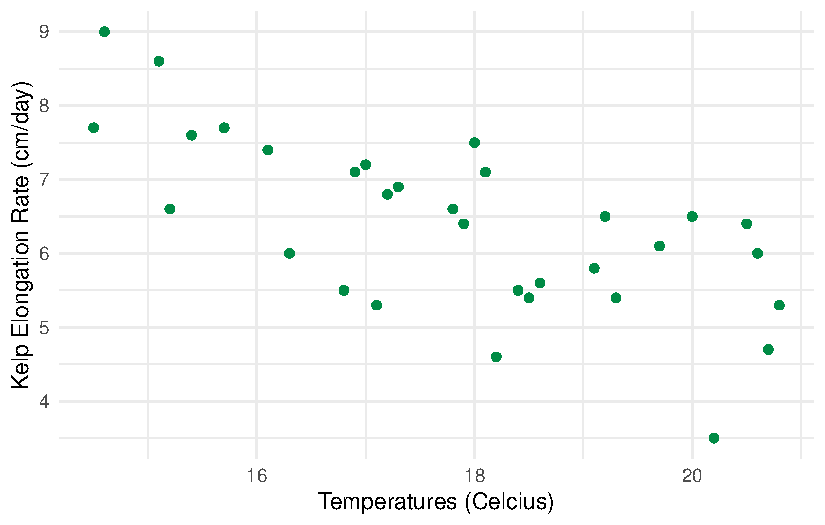
\includegraphics{es193_hw3_codee_files/figure-pdf/unnamed-chunk-3-1.pdf}

\begin{enumerate}
\def\labelenumi{\alph{enumi}.}
\setcounter{enumi}{2}
\tightlist
\item
  Check your assumptions and run your test\newline
\end{enumerate}

\subsubsection{Checking assumptions}\label{checking-assumptions}

\begin{Shaded}
\begin{Highlighting}[]
\CommentTok{\# ggplot as base layer}
\FunctionTok{ggplot}\NormalTok{(}
  \CommentTok{\# using kelp data}
  \AttributeTok{data =}\NormalTok{ kelp,}
  \CommentTok{\# plotting temperature }
  \AttributeTok{mapping =} \FunctionTok{aes}\NormalTok{(}\AttributeTok{sample =}\NormalTok{ temp\_c)}
\NormalTok{) }\SpecialCharTok{+}
  \CommentTok{\# qq line is first layer}
  \FunctionTok{geom\_qq\_line}\NormalTok{() }\SpecialCharTok{+}
  \CommentTok{\# qq points are second layer}
  \CommentTok{\# changing color of the points}
  \FunctionTok{geom\_qq}\NormalTok{(}\AttributeTok{color =} \StringTok{\textquotesingle{}tomato4\textquotesingle{}}\NormalTok{) }\SpecialCharTok{+}
  \CommentTok{\# setting theme as minimal}
  \FunctionTok{theme\_minimal}\NormalTok{()}
\end{Highlighting}
\end{Shaded}

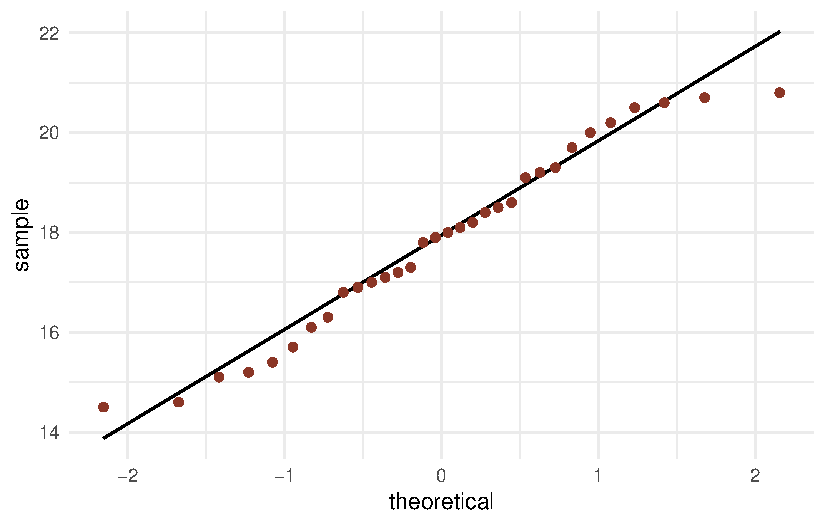
\includegraphics{es193_hw3_codee_files/figure-pdf/unnamed-chunk-4-1.pdf}

\begin{Shaded}
\begin{Highlighting}[]
\CommentTok{\# ggplot as base layer }
\FunctionTok{ggplot}\NormalTok{(}
  \CommentTok{\# using kelp data}
  \AttributeTok{data =}\NormalTok{ kelp,}
  \CommentTok{\# plotting kelp elongation rate}
  \AttributeTok{mapping =} \FunctionTok{aes}\NormalTok{(}\AttributeTok{sample =}\NormalTok{ kelp\_elong)}
\NormalTok{) }\SpecialCharTok{+}
  \CommentTok{\# qq line is first layer}
  \FunctionTok{geom\_qq\_line}\NormalTok{() }\SpecialCharTok{+}
  \CommentTok{\# qq points are second layer}
  \CommentTok{\# changing color of points}
  \FunctionTok{geom\_qq}\NormalTok{(}\AttributeTok{color =} \StringTok{\textquotesingle{}skyblue3\textquotesingle{}}\NormalTok{) }\SpecialCharTok{+}
  \CommentTok{\# setting theme as minimal}
  \FunctionTok{theme\_minimal}\NormalTok{()}
\end{Highlighting}
\end{Shaded}

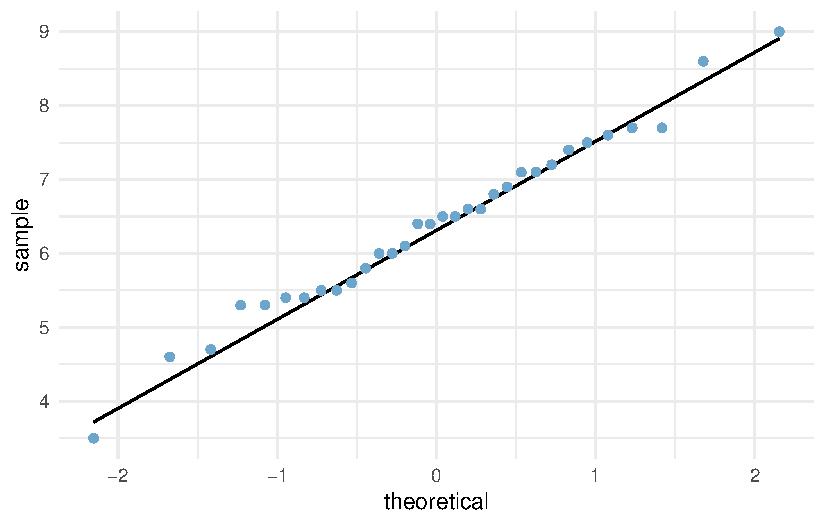
\includegraphics{es193_hw3_codee_files/figure-pdf/unnamed-chunk-4-2.pdf}

I checked the assumption that there is a linear relationship between the
two variables by looking at the scatterplot of temperature and kelp
elongation rate and determined that there is a linear relationship
between them. I checked the assumption that the two variables are
normally distributed by looking at a qq plot for each of the variables.
Since the points are generally around the qq line and are randomly
scattered above and below, I determined that there is a normal
distribution for both variables.

\subsubsection{Running Pearson's Correlation
Test}\label{running-pearsons-correlation-test}

\begin{Shaded}
\begin{Highlighting}[]
\CommentTok{\# running a correlation test}
\FunctionTok{cor.test}\NormalTok{(}
         \CommentTok{\# testing correlation between kelp elongation rate and temperature }
\NormalTok{         kelp}\SpecialCharTok{$}\NormalTok{kelp\_elong, kelp}\SpecialCharTok{$}\NormalTok{temp\_c,}
         \CommentTok{\# method tells you what type of pearson\textquotesingle{}s correlatoin}
         \AttributeTok{method =} \StringTok{"pearson"}\NormalTok{)}
\end{Highlighting}
\end{Shaded}

\begin{verbatim}

    Pearson's product-moment correlation

data:  kelp$kelp_elong and kelp$temp_c
t = -5.189, df = 30, p-value = 1.366e-05
alternative hypothesis: true correlation is not equal to 0
95 percent confidence interval:
 -0.8359665 -0.4460157
sample estimates:
       cor 
-0.6877489 
\end{verbatim}

\begin{enumerate}
\def\labelenumi{\alph{enumi}.}
\setcounter{enumi}{3}
\item
  Results communication\newline To evaluate the strength of the
  relationship between temperature and giant kelp frond elongation rate,
  I used a Pearson's correlation test. We found a moderate negative
  relationship between temperature and kelp frond elongation rate
  (Pearson's correlation, r = -0.6877489, t(30) = -5.189, p = 1.366e-05,
  \(\alpha\) = 0.05).
\item
  Test implications\newline I found that as temperature increases, the
  kelp elongation rate decreases. This is based on my Pearson's
  correlation test, where I found a moderate negative relationship
  between temperatures and kelp frond elongation rate (Pearson's
  correlation, r = -0.6877489, t(30) = -5.189, p = 1.366e-05, \(\alpha\)
  = 0.05). Based on these results we can infer that kelp growth rates
  will be lowered during warmer weather and can be permanently decreased
  due to climate change.
\item
  Double check your own work\newline
\end{enumerate}

\begin{Shaded}
\begin{Highlighting}[]
\CommentTok{\# running spearmans correlation test }
\FunctionTok{cor.test}\NormalTok{(}
  \CommentTok{\# testing correlation between temperature and kelp elongation rate}
\NormalTok{  kelp}\SpecialCharTok{$}\NormalTok{temp\_c, kelp}\SpecialCharTok{$}\NormalTok{kelp\_elong,}
  \CommentTok{\# doing a spearman\textquotesingle{}s correlation}
  \AttributeTok{method =} \StringTok{"spearman"}
\NormalTok{)}
\end{Highlighting}
\end{Shaded}

\begin{verbatim}

    Spearman's rank correlation rho

data:  kelp$temp_c and kelp$kelp_elong
S = 9216.1, p-value = 1.29e-05
alternative hypothesis: true rho is not equal to 0
sample estimates:
       rho 
-0.6891684 
\end{verbatim}

Both the Pearson's correlation test and Spearman's correlation test
would have led me to make the same decision. The Spearman's correlation
test also found a moderate negative relationship between temperature and
kelp frond elongation rates (Spearman's correlation, \(\rho\) =
-0.6891684, S = 9216.1, p = 1.29e-05, \(\alpha\) = 0.05)

\subsection{Problem 2. Personal data}\label{problem-2.-personal-data}

\begin{enumerate}
\def\labelenumi{\alph{enumi}.}
\tightlist
\item
  Updating your visualizations\newline
\end{enumerate}

Cleaning my\_data

\begin{Shaded}
\begin{Highlighting}[]
\CommentTok{\# cleaning my\_data and storing it as object my\_data\_clean}
\NormalTok{my\_data\_clean }\OtherTok{\textless{}{-}}\NormalTok{ my\_data }\SpecialCharTok{|\textgreater{}}
  \CommentTok{\# dropping rows that contain NA values in the computer\_time column}
  \FunctionTok{drop\_na}\NormalTok{(computer\_time) }\SpecialCharTok{|\textgreater{}}
  \CommentTok{\# changing weekday variable inputs}
  \FunctionTok{mutate}\NormalTok{(}\AttributeTok{weekday =} \FunctionTok{case\_when}\NormalTok{(}
    \CommentTok{\# y inputs in the weekday column are now displayed as Weekdays}
    \CommentTok{\# n inputs in the weekday column are not displayed as Weekends}
\NormalTok{    weekday }\SpecialCharTok{==} \StringTok{"y"} \SpecialCharTok{\textasciitilde{}} \StringTok{"Weekdays"}\NormalTok{,}
\NormalTok{    weekday }\SpecialCharTok{==} \StringTok{"n"} \SpecialCharTok{\textasciitilde{}} \StringTok{"Weekends"}
\NormalTok{  ))}

\NormalTok{my\_data\_clean }\OtherTok{\textless{}{-}}\NormalTok{ my\_data\_clean }\SpecialCharTok{|\textgreater{}}
  \FunctionTok{mutate}\NormalTok{(}\AttributeTok{total\_screen\_time =}\NormalTok{ computer\_time }\SpecialCharTok{+}\NormalTok{ phone\_time)}
\end{Highlighting}
\end{Shaded}

\begin{Shaded}
\begin{Highlighting}[]
\CommentTok{\# base layer is ggplot}
\CommentTok{\# data is my\_data\_clean}
\FunctionTok{ggplot}\NormalTok{(}\AttributeTok{data =}\NormalTok{ my\_data\_clean,}
       \CommentTok{\# x axis is whether it is a weekday or weekend}
       \CommentTok{\# y axis is the computer screen time}
       \CommentTok{\# color is based on whether it is the weekday or weekend group}
       \AttributeTok{mapping =} \FunctionTok{aes}\NormalTok{(}\AttributeTok{x =}\NormalTok{ weekday,}
                     \AttributeTok{y =}\NormalTok{ computer\_time,}
                     \AttributeTok{color =}\NormalTok{ weekday)) }\SpecialCharTok{+}
  \CommentTok{\# boxplot is second layer}
  \FunctionTok{geom\_boxplot}\NormalTok{() }\SpecialCharTok{+}
  \CommentTok{\# jitter plot is the third layer}
  \FunctionTok{geom\_jitter}\NormalTok{(}\AttributeTok{shape =} \DecValTok{21}\NormalTok{) }\SpecialCharTok{+}
  \CommentTok{\# renaming y axis, x axis, and title}
  \FunctionTok{labs}\NormalTok{(}\AttributeTok{y =} \StringTok{"Computer Screen Time (minutes)"}\NormalTok{,}
       \AttributeTok{x =} \StringTok{""}\NormalTok{,}
       \AttributeTok{title =} \StringTok{"Weekdays Have Greater Computer Screen Time on Average"}\NormalTok{,}
       \AttributeTok{subtitle =} \StringTok{"05{-}27{-}2026"}\NormalTok{) }\SpecialCharTok{+}
  \CommentTok{\# manually setting color for Weekdays and Weekends gropus}
  \FunctionTok{scale\_color\_manual}\NormalTok{(}\AttributeTok{values =} \FunctionTok{c}\NormalTok{(}\StringTok{"Weekdays"} \OtherTok{=} \StringTok{"dodgerblue3"}\NormalTok{,}
                                \StringTok{"Weekends"} \OtherTok{=} \StringTok{\textquotesingle{}orange2\textquotesingle{}}\NormalTok{)) }\SpecialCharTok{+}
  \CommentTok{\# changing the theme from the default}
  \FunctionTok{theme\_classic}\NormalTok{() }\SpecialCharTok{+}
  \CommentTok{\# removing legend }
  \FunctionTok{theme}\NormalTok{(}\AttributeTok{legend.position =} \StringTok{"none"}\NormalTok{)}
\end{Highlighting}
\end{Shaded}

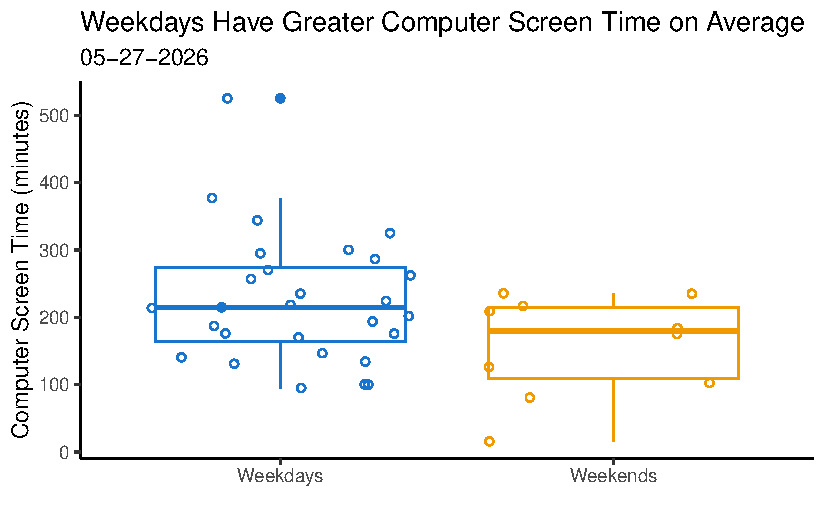
\includegraphics{es193_hw3_codee_files/figure-pdf/unnamed-chunk-8-1.pdf}

\textbf{Figure 1. Weekdays Have Greater Computer Screen Time on
Average}. Hollow blue points represent Weekday daily computer screen
times from April 20, 2026 to May 27, 2026. Hollow orange points Weekend
daily computer screen times from April 20, 2026 to May 27, 2026. The
bottom line of the box represents the 25th percentile, the middle line
represents the median, and the top line represents the 75th percentile.
The lines extended out from the boxplot extend to the furthest point
within 1.5 times the value of the IQR. The filled in point in the
Weekdays group represents an outlier further than 1.5 times the IQR
above the 75th percentile. Data originally from: Jared Umphress. 2026.
Computer Screen Time Data. Data accessed 2026-05-28.

\begin{Shaded}
\begin{Highlighting}[]
\CommentTok{\# ggplot is base layer}
\FunctionTok{ggplot}\NormalTok{(}\AttributeTok{data =}\NormalTok{ my\_data\_clean,}
       \CommentTok{\# x axis is time spent on non computer activities}
       \CommentTok{\# y axis is computer screen time}
       \CommentTok{\# the color of the plot will be orchid4}
       \AttributeTok{mapping =} \FunctionTok{aes}\NormalTok{(}\AttributeTok{x =}\NormalTok{ time\_activities,}
                     \AttributeTok{y =}\NormalTok{ computer\_time}
\NormalTok{                     )) }\SpecialCharTok{+}
  \CommentTok{\# points are second layer}
  \FunctionTok{geom\_point}\NormalTok{(}\AttributeTok{color =} \StringTok{"orchid4"}\NormalTok{) }\SpecialCharTok{+}
  \CommentTok{\# renaming x axis, y axis, and title}
  \FunctionTok{labs}\NormalTok{(}\AttributeTok{x =} \StringTok{"Non{-}Computer Activity Time (minutes)"}\NormalTok{,}
       \AttributeTok{y =} \StringTok{"Computer Screen Time (minutes"}\NormalTok{,}
       \AttributeTok{title =} \StringTok{"Activity Time effect on Computer Screen Time is Unclear"}\NormalTok{,}
       \AttributeTok{subtitle =} \StringTok{"05{-}27{-}2026"}\NormalTok{) }\SpecialCharTok{+}
  \CommentTok{\# changing theme from the default}
  \FunctionTok{theme\_classic}\NormalTok{() }\SpecialCharTok{+}
  \CommentTok{\# removing legend}
  \FunctionTok{theme}\NormalTok{(}\AttributeTok{legend.position =} \StringTok{"none"}\NormalTok{)}
\end{Highlighting}
\end{Shaded}

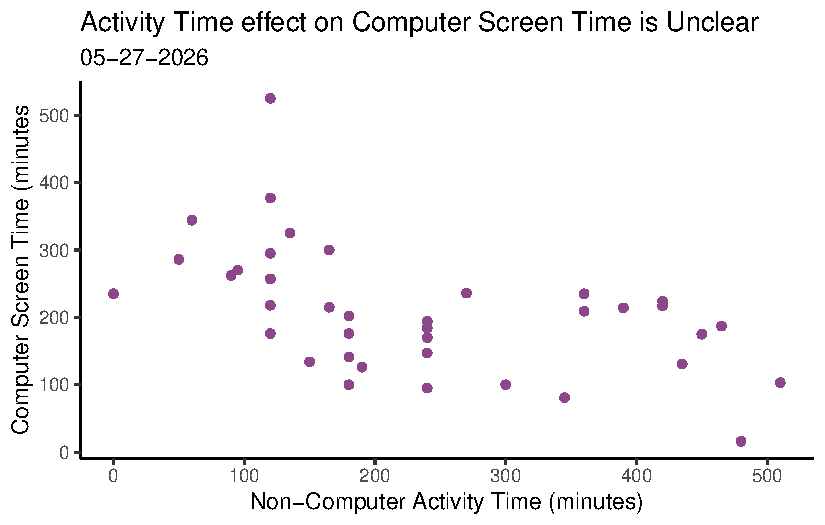
\includegraphics{es193_hw3_codee_files/figure-pdf/unnamed-chunk-9-1.pdf}

\begin{Shaded}
\begin{Highlighting}[]
 \CommentTok{\#theme(legend.position = "none",}
 \CommentTok{\#       panel.grid.major = element\_blank(),}
 \CommentTok{\#        panel.grid.minor = element\_blank(),}
 \CommentTok{\#        panel.background = element\_blank(),}
 \CommentTok{\#        plot.background = element\_blank()}
\end{Highlighting}
\end{Shaded}

\textbf{Figure 3. Computer Screen Time in Relation to Non-Computer
Activity Time.} The filled in purple points represent a given days
Non-Computer Activity Time and Computer Screen Time. Data originally
from: Jared Umphress. 2026. Computer Screen Time Data. Data accessed
2026-05-28.

\begin{enumerate}
\def\labelenumi{\alph{enumi}.}
\setcounter{enumi}{1}
\tightlist
\item
  Captions\newline Captions included above.
\end{enumerate}

\subsection{Problem 3. Affective
visualization}\label{problem-3.-affective-visualization}

\begin{enumerate}
\def\labelenumi{\alph{enumi}.}
\tightlist
\item
  Describe in words what an affective visualization could look like for
  your personal data.\newline
\end{enumerate}

Since I am comparing computer screen time between weekdays vs weekends,
I want to create a dichotomous visual. The weekdays and weekend group
will each have images that combine to form sort of a boxplot. I would
like to frame more computer screen time as bad and less screen time as
good. Since weekdays had higher average computer screen times I want to
use negative meme photos. Since weekends had lower average computer
screen times I want to use positive meme photos.

\begin{enumerate}
\def\labelenumi{\alph{enumi}.}
\setcounter{enumi}{1}
\item
  Create a sketch (on paper) of your idea\newline \begin{center}
  
\includegraphics[width=1\textwidth,height=\textheight]{code/affective_visual_sketch.JPG}
  \end{center}
\item
  Make a draft of your visualization\newline
\end{enumerate}



\end{document}
